\chapter{Level Sets Preservation in $\Lambda \Omega_{2}$ Networks}
\label{sec:results1}
In this section we study whether and under what condition the attribute level sets (LSs) for individual neurons are preserved in $\Lambda \Omega_{2}$ networks. Two $\Lambda \Omega_{2}$ networks with different degree of complexity are considered: the self-connected cell and the two-cell network.

A set of statements, aimed at capturing the main results, are presented in each section.

\section{The self-connected cell}
The set of equations describing the self-connected cell is given by

\begin{equation}
    \frac{dx}{dt} = \lambda x - \omega y - (bx + ay)(x^{2}+y^{2})+\alpha x
    \label{es11_1}
\end{equation}
\begin{equation}
    \frac{dy}{dt} = \omega x + \lambda y + (ax - by)(x^{2}+y^{2})
    \label{es11_2}
\end{equation}

where $\lambda$, $b$, $\omega$ and $a$ are the intrinsic parameters of the cell and $\alpha$ is the self-connectivity parameter.

A necessary condition for the preservation of individual LSs in $\Lambda \Omega_{2}$ networks is that the connectivity matrix has to be singular (see more details in Appendix \ref{sec:appendix}). Therefore, LSs in the self-connected cell will not be preserved.

\begin{Statement}
Attribute level sets are not preserved in the self-connected cell.
\end{Statement}

Fig. (\ref{photo9}) shows the effect of self-inhibition ($\alpha < 0$) and self-excitation ($\alpha > 0$) on different cells belonging to the same individual amplitude and frequency LS for representative parameter values. It is shown how amplitude and frequency are not constant along the individual LS. In particular, the effect of self-inhibition is a decrease in amplitude and frequency, while self-excitation increases both the amplitude and frequency. In both cases, the effect is greater specially for small values of parameter $\lambda$.

\begin{figure}[htb]
\centering
  \begin{minipage}{0.45\linewidth}
  \centering
    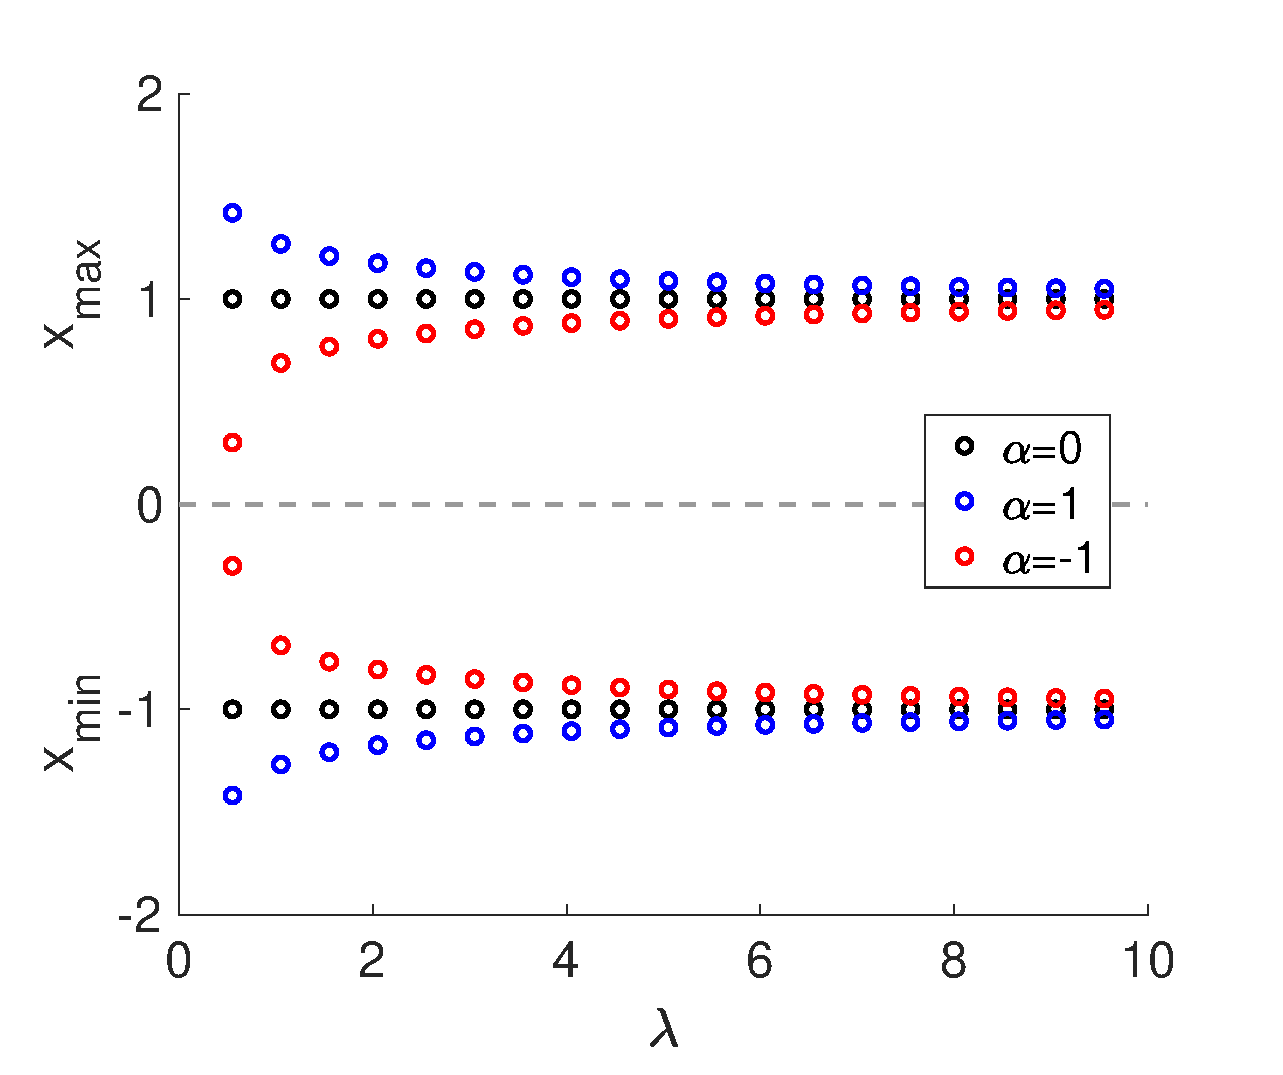
\includegraphics[width=1\linewidth]{Images/photo9_1.eps} 
  \end{minipage} 
  \begin{minipage}{0.45\linewidth}
  \centering
    \includegraphics[width=1\linewidth]{Images/photo9_2.eps} 
  \end{minipage} 
  
  \caption{\textbf{Individual attribute level sets are not preserved in the self-connected cell.} The individual cells belong to the same level set ($K_{a}=1$ and $K_{f}=2$). Left: amplitude envelope diagram as a function of $\lambda$ for representative values of self-connectivity parameter $\alpha$. Right: frequency diagram as a function of $\lambda$ for representative values of self-connectivity parameter $\alpha$. Parameter values: $a = 1$ and $\omega = 1$.}
  \label{photo9}
\end{figure}

\section{The Two-cell Network}
The set of equations describing the self-connected cell are given by

\begin{equation}
    \frac{dx_{1}}{dt} = \lambda_{1} x_{1} - \omega_{1} y_{1} - (b_{1}x_{1} + a_{1}y_{1})(x_{1}^{2}+y_{1}^{2}) + \alpha_{11}x_{1} + \alpha_{12}x_{2}
    \label{es121}
\end{equation}
\begin{equation}
  \frac{dy_{1}}{dt} = \omega_{1} x_{1} + \lambda_{1} y_{1} + (a_{1}x_{1} - b_{1}y_{1})(x_{1}^{2}+y_{1}^{2})
   \label{es122}
\end{equation}

\begin{equation}
    \frac{dx_{2}}{dt} = \lambda_{2} x_{2} - \omega_{2} y_{2} - (b_{2}x_{2} + a_{2}y_{2})(x_{2}^{2}+y_{2}^{2}) + \alpha_{21}x_{1} + \alpha_{22}x_{2}
     \label{es123}
\end{equation}
\begin{equation}
  \frac{dy_{2}}{dt} = \omega_{2} x_{2} + \lambda_{2} y_{2} + (a_{2}x_{2} - b_{2}y_{2})(x_{2}^{2}+y_{2}^{2})
   \label{es124}
\end{equation}

where $\lambda_{i}$, $b_{i}$, $\omega_{i}$ and $a_{i}$ ($i=1,2$) are the intrinsic parameters of the cells and $\{\alpha_{ij}\}_{i,j=1,2}$ is the connectivity matrix whose coefficients are the connectivity parameters.

We show that there exist conditions for individual LSs preservation in the two-cell network. In particular there exist 2-dimensional manifolds on connectivity parameter space which preserve individual LSs, provided individual cells belong to the same frequency LS.

Furthermore, analytical expression for these manifolds can be written down. We proceed as follows. Firstly, necessary and sufficient conditions for the existence of an individual limit circle in each cell are found. Under these conditions, each cell shows an individual limit circle for 2-dimensional manifolds on connectivity parameter space.

We notice that the existence of an individual limit circle in each cell is not sufficient for LSs preservation, since limit circles should be stable in order to show sustained oscillations. Then, we obtain (computationally) restricted 2-dimensional manifolds which preserve individual LSs. (see more details in Appendix \ref{sec:appendix}).

As a result, connectivity matrices preserving individual LSs can be found both in homogeneous and heterogeneous networks. In the following we summarize conditions for LSs preservation.

\begin{Statement} 
Individual cells must belong to the same frequency level set ($K_{f}$) in order to preserve attribute level sets. Therefore, heterogeneous networks in which cells belong to different frequency level sets do not preserve individual attribute level sets.
\end{Statement}

Taking into account the analytical expressions of amplitude and frequency LSs in $\Lambda \Omega_{2}$ systems, in the most general situation in which cells belong to different amplitude LSs ($K_{a1}$ and $K_{a2}$), intrinsic parameters $\omega_{1}$, $\omega_{2}$, $a_{1}$ and $a_{2}$ must verify the condition

\begin{equation}
    \omega_{1}+a_{1}K_{a1} = \omega_{2}+ a_{2}K_{a2}
    \label{es125}
\end{equation}

in order to belong to the same individual frequency LS.

\begin{Statement} 
Homogeneous and heterogeneous (cells belong to different individual amplitude level sets) two-cell networks preserve individual attribute level sets on 2-dimensional manifolds on connectivity parameter space. 
\end{Statement} 

We have found that there are two types of networks which preserve individual LSs, namely synchronized and non-synchronized networks. In synchronized networks, cells oscillate in phase ($\Delta \varphi = 0$), whereas in non-synchronized networks, cells oscillate in antiphase ($\Delta \varphi = \pm \pi$). Whether the network which preserve individual LSs is synchronized or not does depend on cross-connectivity parameters.

The following statement summarizes the possible networks according to the inhibitory (negative value) or excitatory (positive value) character of connectivity parameters. 

\begin{Statement} 
Mutually excitatory and inhibitory cross-connectivity under self-inhibition preserve level sets in the two-cell network. Mutually excitatory cross-connectivity leads to synchronized networks whereas mutually inhibitory cross-connectivity leads to non-synchronized networks.
\end{Statement} 

In order to compute closed matrix forms preserving individual LSs, we define the additional parameter

\begin{equation}
    \gamma = \frac{\bar{r_{1}}}{\bar{r_{2}}}
\end{equation}

where 

\begin{equation}
    \bar{r_{1}} = \sqrt{\frac{\lambda_{1}}{b_{1}}}  \hspace{0.5cm} \text{and} \hspace{0.5cm} \bar{r_{2}} = \sqrt{\frac{\lambda_{2}}{b_{2}}}
    \label{e28}
\end{equation}

are the amplitude value of cell-1 and cell-2 respectively. We note that parameter $\gamma$ has value one when cells are either identical (homogeneous networks) or belong to the same individual amplitude (and also frequency) LSs (type-\textrm{I} heterogeneous networks). In contrast, it has a different values when cells belong to different individual amplitude LSs (type-\textrm{II} heterogeneous networks).

\subsection{Non-Synchronized Networks Preserving Level Sets}
\begin{Statement} 
Connectivity matrices with the general form

\begin{equation}
   C_{\text{non-syn}} = 
    \begin{pmatrix}
        -\gamma^{-1}\alpha & -\alpha\\
        -\beta & -\gamma \beta
    \end{pmatrix}
    \text{ , } \hspace{0.5cm} \alpha, \beta \geq 0
    \label{e30}
\end{equation}

do preserve attribute LSs both in type-\textrm{I} heterogeneous (cells belong to the same amplitude and frequency LS) and type-\textrm{II} heterogeneous (cells belong to the different amplitude LSs) provided cells belong to the same frequency LS.
Furthermore networks are non-synchronized.
\end{Statement} 

Fig. (\ref{photo11}) shows voltage traces in a non-synchronized network preserving individual LSs. It is also shown how individual LSs of cell-1 are preserved in the network.

\begin{figure}[htb]
   \begin{minipage}{0.32\linewidth}
            \begin{center}
                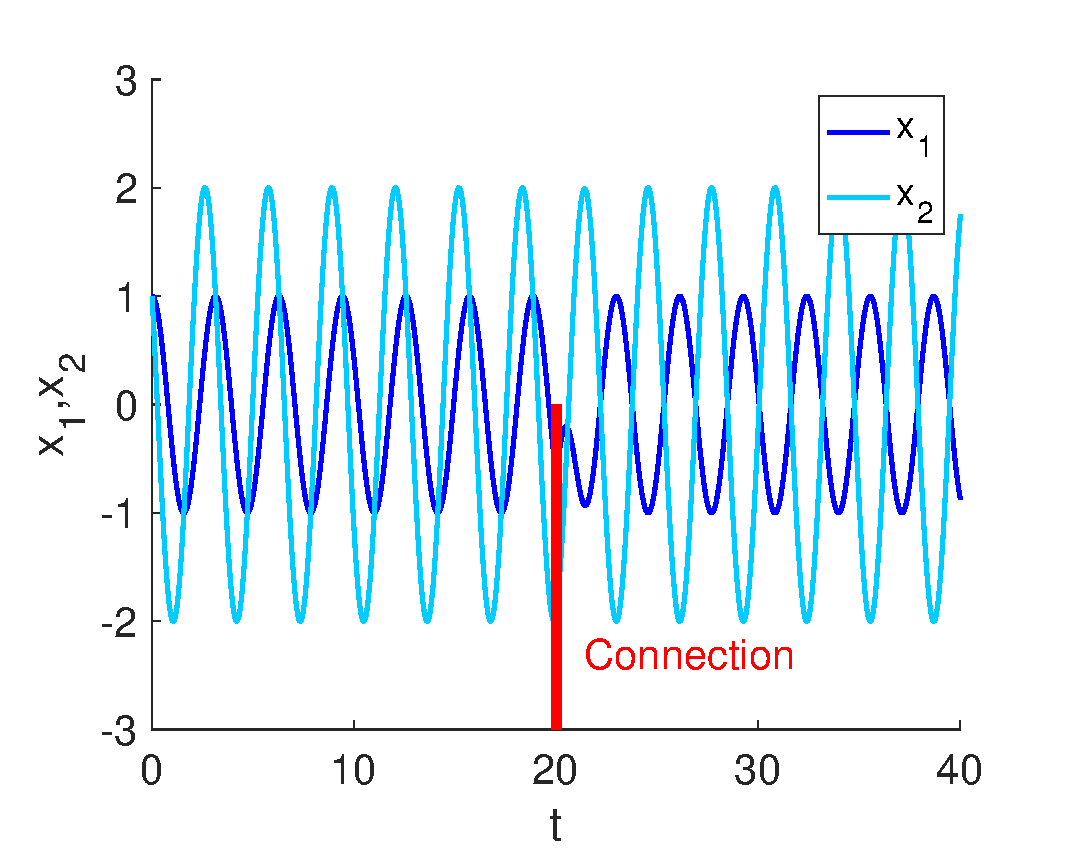
\includegraphics[width=1\linewidth]{Images/photo11_1.eps}
            \end{center}
        \end{minipage} 
        \begin{minipage}{0.32\linewidth}
            \begin{center}
                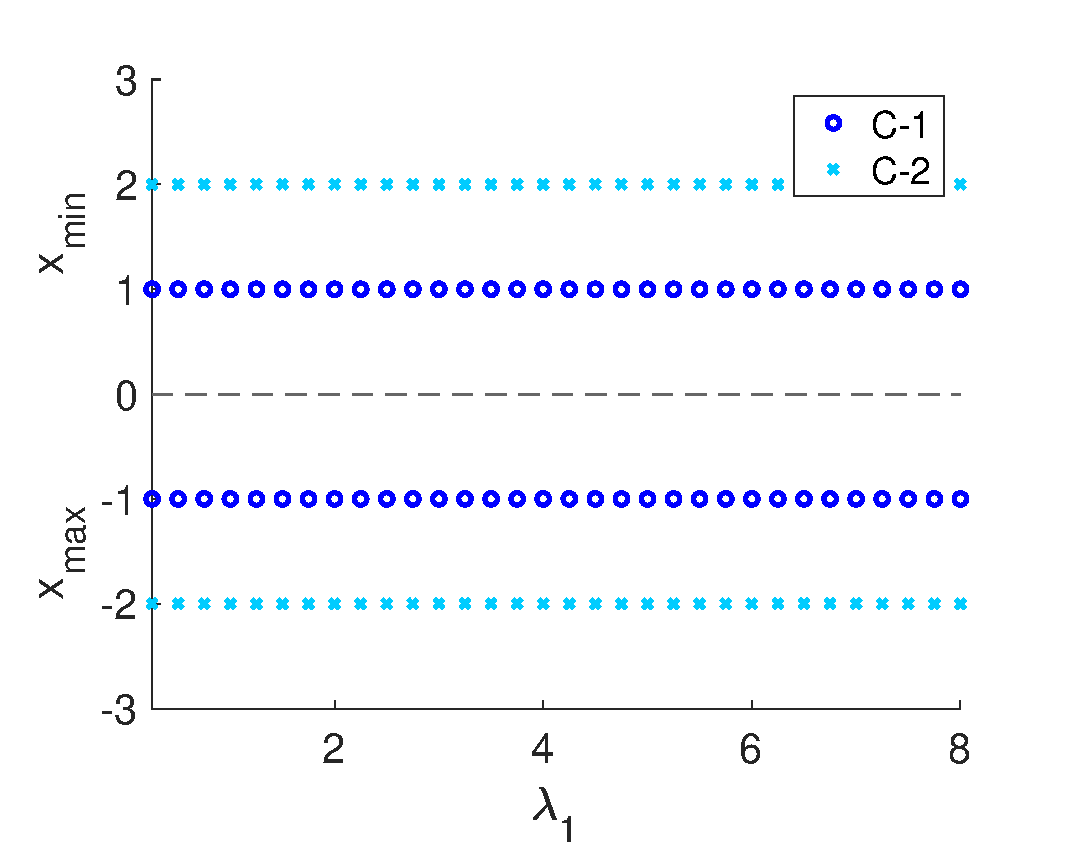
\includegraphics[width=1\linewidth]{Images/photo10_2.eps}
            \end{center}
        \end{minipage} 
    \begin{minipage}{0.32\linewidth}
        \begin{center}
            \includegraphics[width=1\linewidth]{Images/photo10_3.eps}
        \end{center}
    \end{minipage} 
  \caption{\textbf{Non-Synchronized network preserving individual attribute level sets.} Left: voltage traces $x_{1}$ and $x_{2}$ before and after the connection. Vertical Red line indicates the time at which cells form the network. Middle: amplitude envelope diagram for values $(\lambda_{1},b_{1})$ belonging to the same individual amplitude level set ($K_{a,1}=1$). Left: frequency diagram for values $(\lambda_{1},b_{1})$ belonging to the same individual amplitude level set ($K_{a,1}=1$). Parameter values: $a_{1} = 1$, $\omega_{1} = 1$, $a_{2}=1/4$, $\omega_{2} = 1$, $\gamma = 1/2$, $\alpha = 1$ and $\beta=1$.}
  \label{photo11}
\end{figure}

\subsection{Synchronized Networks Preserving Level Sets}
\begin{Statement} 
Connectivity matrices with the general form
\begin{equation}
   C_{\text{syn}} = 
    \begin{pmatrix}
        -\gamma^{-1}\alpha & \alpha\\
        \beta & -\gamma \beta
    \end{pmatrix}
    \text{ , } \hspace{0.5cm} \alpha, \beta \geq 0
    \label{e29}
\end{equation}
do preserve attribute level set both in type-\textrm{I} heterogeneous (cells belong to the same amplitude and frequency LS) and type-\textrm{II} heterogeneous (cells belong to the different amplitude LSs) provided cells belong to the same frequency level set . Furthermore networks are synchronized.
\end{Statement} 

Fig. (\ref{photo10}) shows voltage traces in a synchronized network preserving individual attributes LSs. It is also shown how individual LSs of cell-1 are preserved in the network.

 \begin{figure}[htb]
        \begin{minipage}{0.32\linewidth}
            \begin{center}
                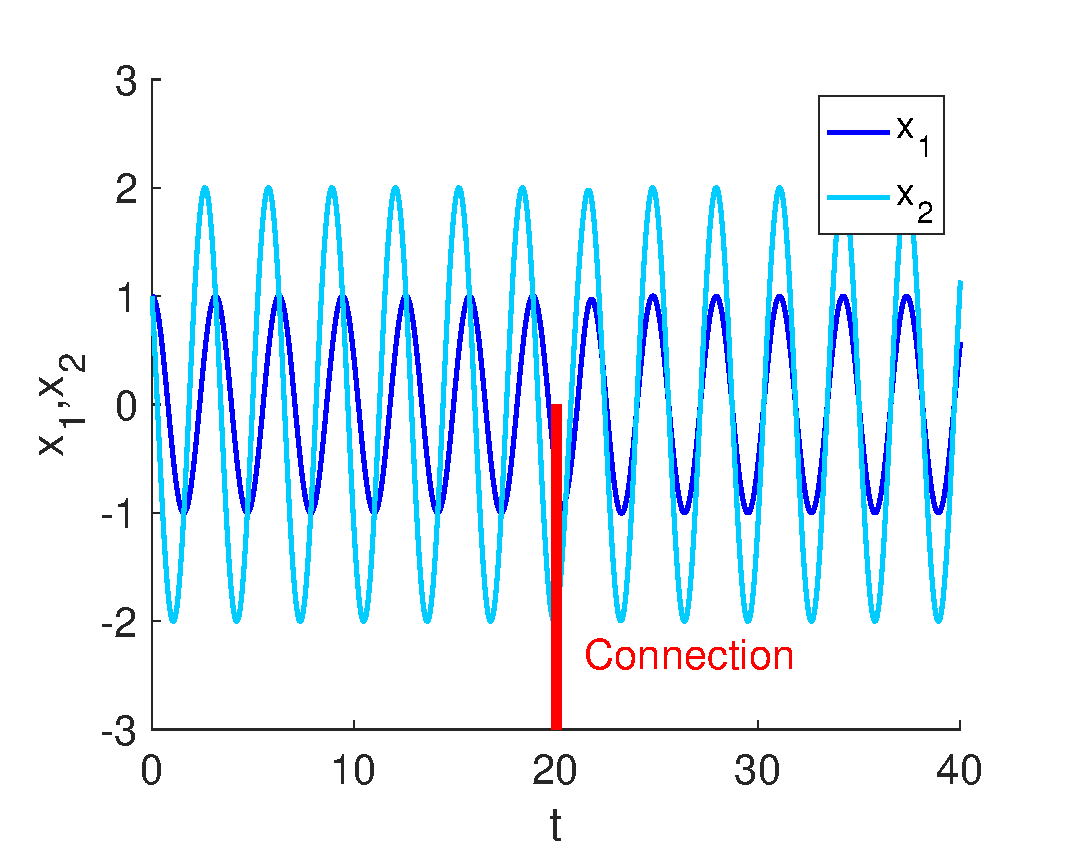
\includegraphics[width=1\linewidth]{Images/photo10_1.eps}
            \end{center}
        \end{minipage} 
        \begin{minipage}{0.32\linewidth}
            \begin{center}
                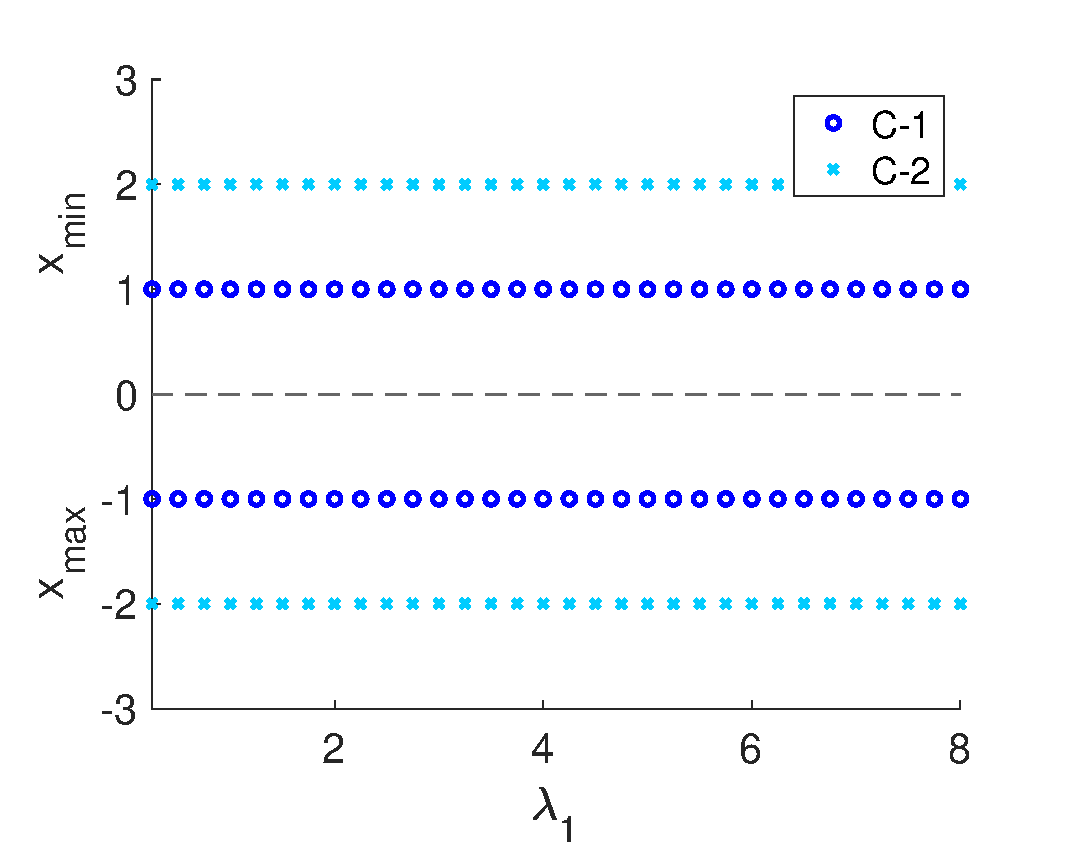
\includegraphics[width=1\linewidth]{Images/photo10_2.eps}
            \end{center}
        \end{minipage} 
    \begin{minipage}{0.32\linewidth}
        \begin{center}
            \includegraphics[width=1\linewidth]{Images/photo10_3.eps}
        \end{center}
    \end{minipage} 
  
  \caption{\textbf{Synchronized network preserving individual attribute level sets.} Left: voltage traces $x_{1}$ and $x_{2}$ before and after the connection. Vertical Red line indicates the time at which cells form the network. Middle: amplitude envelope diagram for values $(\lambda_{1},b_{1})$ belonging to the same individual amplitude level set ($K_{a,1}=1$). Left: frequency diagram for values $(\lambda_{1},b_{1})$ belonging to the same individual amplitude level set ($K_{a,1}=1$). Parameter values: $a_{1} = 1$, $\omega_{1} = 1$, $a_{2}=1/4$, $\omega_{2} = 1$, $\gamma = 1/2$, $\alpha = 1$ and $\beta=1$.}
  \label{photo10}
\end{figure}

\subsubsection{Gap-Junctions: Synchronized Electrical Network Preserving Level Sets}

We highlight synchronized type-I heterogeneous networks, which preserve individual LSs. In this case, matrices preserving individual LSs has the general form

\begin{equation}
   C_{\text{gap-juntion}} = 
    \begin{pmatrix}
        -\alpha & \alpha\\
        \beta & -\beta
    \end{pmatrix}
    \text{ , } \hspace{0.5cm} \alpha, \beta \geq 0
\end{equation}

This kind of connectivity would corresponds to the case where cells are coupled through electrical synapses or gap junctions. In realistic neuron network models, electrical synapses would produce a synaptic current proportional to the difference between the pre- and post-synpatic membrane potentials, \cite{book1}.

\begin{Statement} 
Gap juntions preserve level sets in type-\textrm{I} heterogeneous networks where cells belong to the same amplitude and frequency level set. However, gap-junctions do not preserve individual level sets in type-\textrm{II} heterogeneous networks.
\end{Statement}
